The infrastructure that currently serves the Drupal websites can be seen in figure \ref{fig:drupal-physical-request-journey}.
It runs on CentOS 7 and uses Puppet for configuration management.
All servers run the same environment with systemd services, some of which are:
\begin{itemize}
    \item HAProxy load balancer: routes requests to worker nodes, with an affinity cookie
    \item Keepalived: floating IP for the load balancer
    \item Apache httpd: serves Drupal PHP code, WebDAV interface and a few additional PHP management applications
    \item php-fpm: maintains a pool of worker processes that generate Drupal content
\end{itemize}

\subsection{Request journey}

The journey of an HTTP request can be seen in figure \ref{fig:drupal-physical-request-journey}.
Production websites respond to the load by spawning PHP workers, up to a maximum of 25.
A worker process is always listening for requests, even without load.
Test websites, on the other hand, spawn the first worker on demand and scale up to a maximum of 10 workers.
The PHP memory limit for every website is 512MB.

\begin{wrapfigure}{r}{.62\textwidth}
    \vspace{-4em}
    \centering
    \hspace{-2em}
    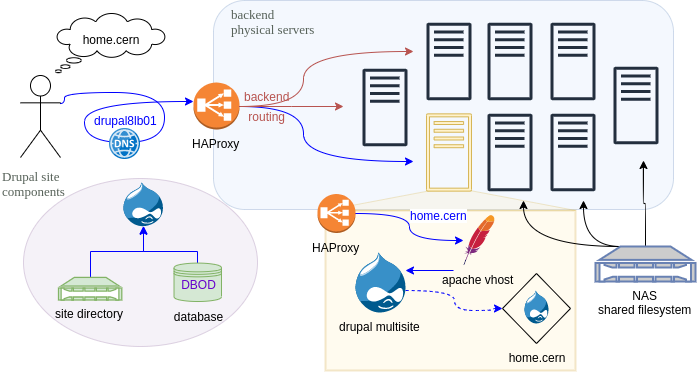
\includegraphics[width=.66\textwidth]{figures/drupal-physical-request-journey}
    \caption{\emph{Request journey in the physical infrastructure}.
    The infrastructure consists of 8 physical Linux servers behind a floating IP, equipped with NAS storage.
    The {\color{blue} datapath} to access a site is shown in blue. 
    Drupal is configured in multisite mode to look up a separate directory and database for each site.
    The website's {\color{asparagus} 2 data components}: a persistent directory on the NAS and a database on an external service (DBOD).
    }
    \vspace{-2em}
    \label{fig:drupal-physical-request-journey}
\end{wrapfigure}

\subsection{Website isolation}

Weak isolation is one of the biggest concerns of this infrastructure.
Each website is assigned a Linux user.
Its directory is owned by it and not accessible by the users of other websites.
When Apache serves a request, it \texttt{chroots} the PHP process into the Drupal directory and sets the website's user.
This distinction provides a basic isolation mechanism.

Nevertheless, websites are coupled in many places.
We've never detected a cross-site security incident,
but there are no \texttt{cgroup} limits to resources, and not enough security layers to defend against privilege escalation exploits.
This is a critical concern, given the vulnerability of CMS software \cite{shteimanWhyCMSPlatforms2014},
and the impact that defacing a high-traffic public site would have to CERN's reputation.

A fundamental security practice is rapidly update upon security releases \cite{csontosAccessibilityUsabilitySecurity2021},
but updating the multisite environment is fraught with dangers.
All websites need to be updated in a massive, forced upgrade campaign, and if any has errors, it needs rapid debugging.
Errors are supposed to be detected in a test environment, but not every website has one.

Furthermore, even though websites can be customized with contributed modules, there is no workflow to version control the websites.

\subsection{Development workflow}

Two types of website are supported administratively, corresponding to different Quality of Service (QoS) expectations: official (production) and test (test and development).
There is no concept of \emph{\lq\lq environments\rq\rq} or branches in this infrastructure. Developing a website involves maintaining a production website and one or more independent development websites.
Data can be cloned between websites, so that the development website reproduce the production one.

A site admin that wants to safely develop a new content type or view, add a new module, or even change configuration, should start by cloning the production website to a development website.
They need to keep track of changes, then reproduce them on the production website.
There is no GitOps.

Despite seeming inefficient from a software engineering perspective, this workflow is acceptable by most website admins.
The ones with development experience though would benefit significantly from version controlling configuration changes and extra modules.

\subsection{Limitations of the current infrastructure}
\label{sec-limitations}

Reiterating the discussion, these are the major limitations of the current infrastructure.
In section \ref{sec-k8s-design}, the Kubernetes infrastructure lifts all of them.

\begin{itemize}
    \item Hard to adapt resources, resulting in massive under-utilization
    \item Not very fault tolerant
    \item Weak site isolation increases the risk of severe security incidents affecting multiple sites
    \item Inflexible website environment limits development \& testing workflows, makes upgrades cumbersome 
    \item \emph{Technical debt}: a lot of homebrew components built with legacy technologies specific to this system.
          Far from industry standards.
\end{itemize}
